\documentclass[twoside]{article}
\usepackage{../quiz}
\usepackage{fancyhdr}

\pagestyle{fancy}
\renewcommand{\headrulewidth}{0pt}
\cfoot{}
\rfoot{Solutions to these quizzes will be posted at \textbf{\href{http://owenjow.xyz/cs61a/section-quizzes/}{owenjow.xyz/cs61a/section-quizzes}}.}
\renewcommand{\footrulewidth}{0.4pt}

\lstset{
    language=Python,
    basicstyle=\ttfamily,
    showstringspaces=false
    keywordstyle=\color{black},
    commentstyle=\color{black},
    stringstyle=\color{black},
    escapeinside={<*}{*>},
}

\def\semester{Spring 2k17}
\newcommand{\solution}[1]{{\color{red}#1}}

%%% Actual, flexible content begins here %%%
\title{\sc Quiz 2 \solution{Solutions}}

\begin{document}
\maketitle

\begin{enumerate}
%%% Q1 %%%
\q{10}{Beasts of All Natures}

Draw the environment diagram that results from executing the code below (until the entire program is finished, or an error occurs).
\vspace{0.1in}

\begin{lstlisting}
x = 6
def dread(pirate):
    x = 10
    def roberts(westley):
        x = 2000
        return westley + pirate(x)
    return roberts(x)

dread(lambda spot: x + spot)
\end{lstlisting}

\begin{figure}[ht!]
\hspace*{5mm}
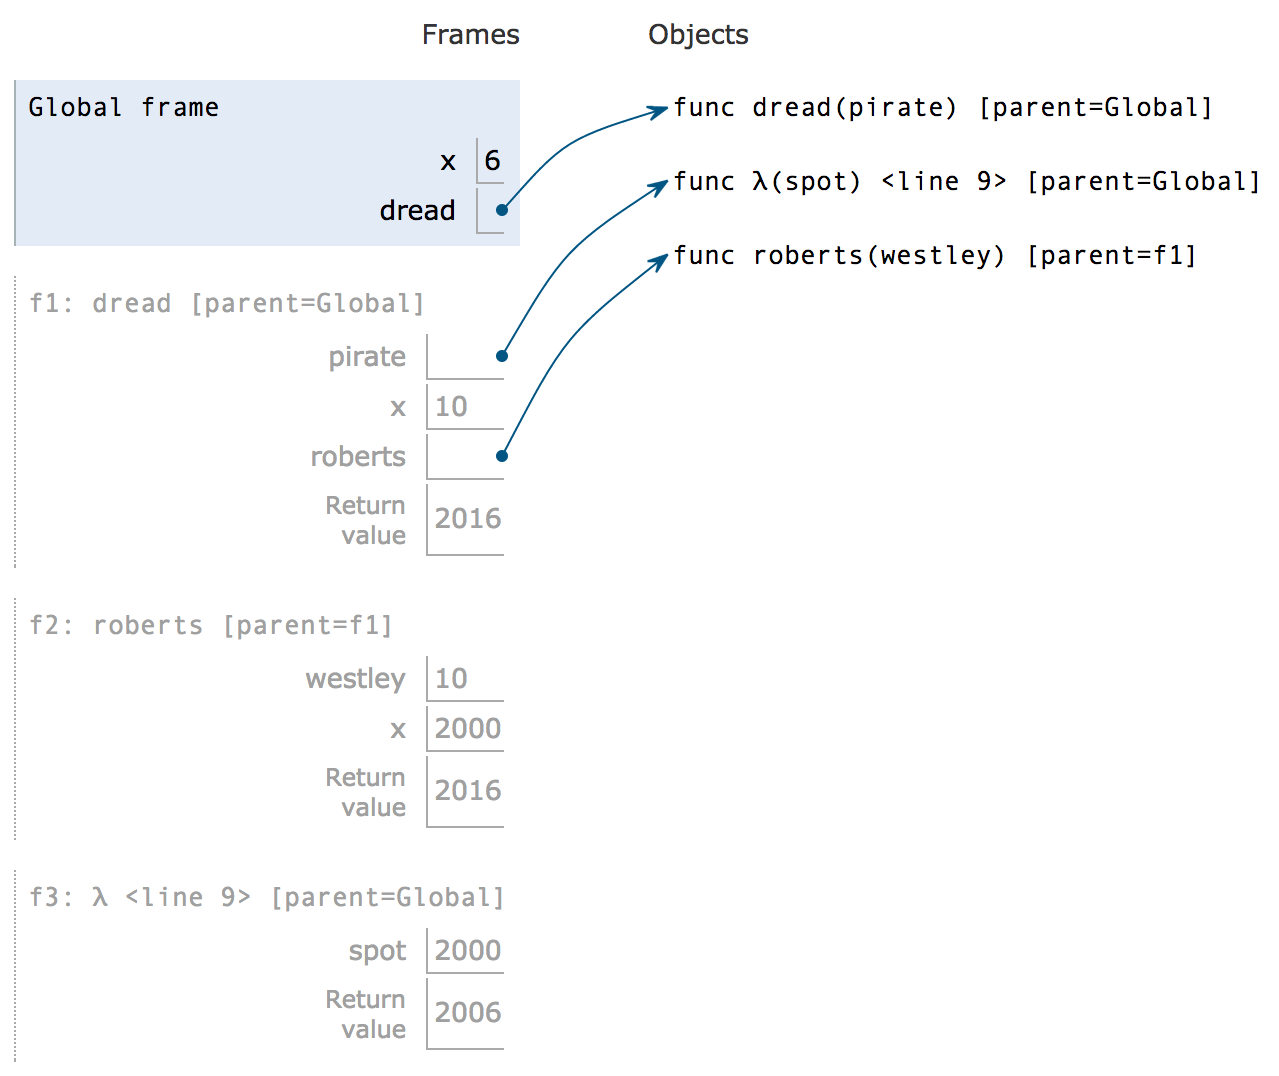
\includegraphics[width=155mm]{../../../../images/quiz2_sol.png}
\end{figure}

\end{enumerate}
\end{document}
